\documentclass[a4paper]{article}
\usepackage[margin=1in]{geometry} % 设置边距,符合Word设定
\usepackage{ctex}
\usepackage{url}
\usepackage{graphicX}
% Keywords command
\providecommand{\keywords}[1]
{
    \small	
    \textbf{关键词:} #1
}

% Keywords command
\providecommand{\keywords}[1]
{
  \small	
  % \textbf{\textit{Keywords---}} #1
  \textbf{关键词:} #1
}
\title{\heiti\zihao{3} 椭圆曲线公钥密码算法的数学原理分析}
\date{班级:2022211805  学号:2022211576  姓名:崔航}
% \author{\songti 崔航}
\begin{document}
    \maketitle
\begin{abstract}
ECC 是 Elliptic Curves Cryptography 的缩写,意为椭圆曲线密码编码学,是基于椭圆曲线数学理论实现的一种非对称加密算法,最初由Koblitz
和Miller两人于1985年提出。相比于RSA,ECC使用更短的密钥,实现与RSA相当或更高的安全的一种信息加密算法。
\end{abstract}
\keywords{群、椭圆曲线、ECC、加解密}
\tableofcontents
\section{阿贝尔群}
椭圆曲线的运算是在一个阿贝尔群上进行的,所以我们先来了解一下阿贝尔群的定义。
\subsection{概念及特征}
加群是一个集合,集合中的元素可以进行加法运算,且满足以下条件:
\begin{itemize}
\item 封闭性:对于任意的$a,b\in G$,有$a+b\in G$。
\item 结合律:对于任意的$a,b,c\in G$,有$(a+b)+c=a+(b+c)$。
\item 单位元:存在一个元素$e\in G$,使得对于任意的$a\in G$,有$a+e=e+a=a$。
\item 逆元:对于任意的$a\in G$,存在一个元素$-a\in G$,使得$a+(-a)=(-a)+a=0$。
\end{itemize}
阿贝尔群是一个加群,且满足交换律,即对于任意的$a,b\in G$,有$a+b=b+a$。



\section{椭圆曲线}
一条椭圆曲线是在射影平面上满足威尔斯特拉斯方程(Weierstrass)所有点的集合,仅仅是形式上的称呼,与椭圆没有关系。
$$Y^{2}Z+a_{1}XYZ+a_{3}YZ^{2}=X^{3}+a_{2}X^{2}Z+a_{4}XZ^{2}+a_{6}Z^{3}$$
\indent 1. 椭圆曲线方程是一个齐次方程\\
\indent 2. 曲线上的每个点都必须是非奇异的(光滑的),偏导数FX(X,Y,Z)、FY(X,Y,Z)、FZ(X,Y,Z)不同为0\\
\indent 3. 圆曲线的形状,并不是椭圆的。只是因为椭圆曲线的描述方程,类似于计算一个椭圆周长的方程故得名\\

最简单的椭圆曲线方程为$y^2=x^3+ax+b$,其中$a,b$为常数,$x,y$为变量。针对曲线$Ep(a,b)$表示为$y^2=x^3+ax+b\bmod p$,其中$4a^{3}+27b^{2}\not =0$,$x,y\in [0,p-1]$,$p$为质数。\\
\\
\subsection{椭圆曲线的加法}:
\\
任取椭圆曲线上的不同两点$P$和$Q$(相同时,取切线),且$P\not =-Q$,过$P$和$Q$的直线与椭圆曲线相交于另一点$R$,则$P+Q=R$。\\


\begin{figure}[htbp]
    \centering
    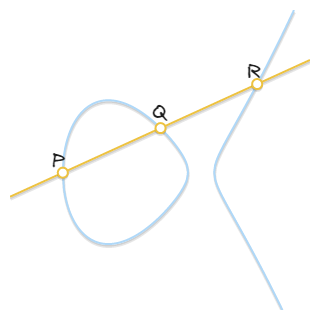
\includegraphics[width=0.4\textwidth]{ECC_add_01.png}
    \caption{椭圆曲线的加法}
    \label{fig:1}

\end{figure}
作$R$关于$x$轴的对称点$R'$,则$P+Q=R'$。\\
\begin{figure}[htbp]
    \centering
    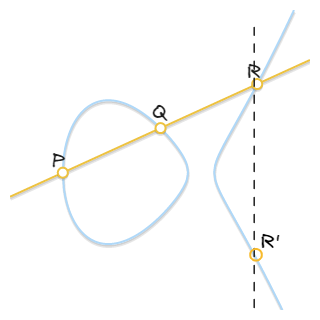
\includegraphics[width=0.4\textwidth]{ECC_add_02.png}
    \caption{椭圆曲线的加法}
    \label{fig:2}
    
\end{figure}
\\
\indent 综上,$P+Q+R=0$。\\
\subsection{椭圆曲线的逆元}
在实数域$R$上的椭圆曲线中,点$P(x_{P},y_{P})$的逆元为与$P$关于$x$轴对称的点$P'(x_{P},-y_{P})$。\\
\\
\subsection{椭圆曲线的阶}
如果椭圆曲线上的点$P$存在最小的正整数$n$,使得$nP=0$,则称$n$为椭圆曲线的阶。\\

\section{ECC}
\subsection{过程步骤}
设私钥为$k$,公钥为$Q$,基点为$G$,则有$Q=dG$。\\
\indent 1. 选择一条椭圆曲线$E$,并选取一个基点$G$,基点的阶为$n$\\
\indent 2. 选择一个私钥$k$,计算公钥$Q=kG$\\
\indent 3. 将$E$、$n$、$G$、$Q$公开,保密$k$\\
\indent 4. 加密时,选择一个随机数$r$,计算$C_1=rG$,$C_2=M+rQ$\\
\indent 5. 解密时,计算$C_2-kC_1$\\

\subsection{ECC的安全性}
ECC的安全性基于椭圆曲线离散对数问题,即给定$E$、$n$、$G$、$Q$,求$k$。
当椭圆曲线上的素数$p$选的比较大时,有$k$和$P$,容易求出$Q=kP$。相反,有$Q$和$P$,是难以求出$k$的。
\section{ECC加解密实例}
\subsection{情景描述} 
\begin{enumerate}
    \item 取$p=11,E_{p}=(1,6)$,椭圆曲线为$y^2=x^3+x+6\pmod{11}$。$E_{p}$的一个生成元为$\alpha=G=(2,7)$,$B$的私钥为$k=7$,假设$A$要发送消息$m=(10,9)$给$B$。求加解密过程。
    \item 密钥生成:$K=kG=7(2,7)=(7,2)$,$B$的公钥为$\{E:y^{2}\equiv x^{3}+x+6\pmod{11},\alpha=G=(2,7),K=(7,2)\}$。
    \item 加密过程:$A$选择随机数$r=3$,计算$C_{1}=rG=3(2,7)=(8,3)$,$C_{2}=m+rK=(10,9)+3(7,2)=(10,2)$。$A$将密文$(C_{1},C_{2})$发送给$B$。  
    \item 解密过程:$B$计算$C_{2}-kC_{1}=(10,2)-7(8,3)=(10,2)-7(8,3=(10,9)$。$B$得到明文$m=(10,9)$。    
\end{enumerate}
\subsection{python算法实现}

\begin{verbatim}
    def get_points(a, b, p):
    """
     获取有限域下的散点集
    """
    # 计算所有可能的点坐标
    points = []
    for x in range(p):
        y_square = (x ** 3 + a * x + b) % p
        for y in range(p):
            if (y ** 2) % p == y_square:
                points.append((x, y))
    return points


def cal_k(point_A, point_B, p):
    """
    计算斜率k
    """
    if point_A == point_B:
        son = 3 * pow(point_A[0], 2) + a
        mother = 2 * point_A[1]
        # 费马小定理求分数取模
        return (son * pow(mother, p - 2)) % p

    else:
        son = point_B[1] - point_A[1]
        mother = point_B[0] - point_A[0]
        # 费马小定理求分数取模
        return (son * pow(mother, p - 2)) % p


def cal_add(point_A, point_B, p, k):
    """
     椭圆曲线加法
     计算A+B的结果坐标
    :param k: 斜率
    """
    # A+B=C,计算c的坐标
    cx = (k ** 2 - point_A[0] - point_B[0]) % p
    cy = (k * (point_A[0] - cx) - point_A[1]) % p
    return cx, cy


def cal_NA(key, point_A, point_B, p):
    """
    椭圆曲线乘法
    计算NA
    """
    # 执行0~key-1共key次
    for i in range(key - 1):
        k = cal_k(point_A, point_B, p)
        point_B = cal_add(point_A, point_B, p, k)

    return point_B


def encryption(r, Q, m, p):
    """
   加密
    """
    cx = cal_NA(r, A, B, p)
    rQ = cal_NA(r, Q, Q, p)
    k = cal_k(m, rQ, p)
    cy = cal_add(m, rQ, p, k)
    return cx, cy


def decryption(cplantext, key, p):
    """
    解密
    """
    kc2 = cal_NA(key, cplantext[0], cplantext[0], p)
    # 减法即关于x轴对称点的坐标
    kc2 = (kc2[0], -kc2[1])
    k = cal_k(cplantext[1], kc2, p)
    result = cal_add(cplantext[1], kc2, p, k)
    return result


# 测试-------------------------------------------------------------------
# 椭圆曲线的a,b
a = 1
b = 6
# 有限域的阶
p = 11
# 私钥k
key = 7
# 散点表
points = get_points(a, b, p)
print("散点表中的元素:")
print(points, end='')
print("\n-------------------------------------------------------------------")
# ------------------------------------------------------------------------
# A是基点,为散点表中的一点,B是另一个交点,这里初始时相同
A = (2, 7)
B = (2, 7)
# 公钥Q=7A
Q = cal_NA(key, A, B, p)
# 随机数r
r = 3
# --------------------------------------------------------------------------
# 消息
message = (10, 9)
print(f"原始消息:{message}")
# 密文
c = encryption(r, Q, message, p)
print(f"加密后的结果:{c}")
# 解密
result = decryption(c, key, p)
print(f"解密后的结果:{result}")


\end{verbatim}
\section{ECC的实际应用}
\begin{itemize}
    \item 电子签名
    \item 数字版权
    \item 数字现金
    \item 数字证书
    \item 密钥协商
    \item 软件认证
    \item IP设计
\end{itemize}
\section{总结}
ECC 算法的数学理论非常深奥和复杂,在工程应用中比较难于实现,但它的单位安全强度相对较高,它的破译或求解难度基本上是指数级的,黑客很难用通常使用的暴力破解的方法来破解。RSA算法的特点之一是数学原理相对简单,在工程应用中比较易于实现,但它的单位安全强度相对较低。因此,ECC算法的可以用较少的计算能力提供比RSA加密算法更高的安全强度,有效地解决了“提高安全强度必须增加密钥长度”的工程实现问题。
\begin{thebibliography}{1000}  
    
    \bibitem{ref1}墨城烟柳ベ旧人殇. ECC加密算法详解+python实现. (2023.07.07). \\\url{https://blog.csdn.net/weixin_51496226/article/details/131320249}
    \bibitem{ref2}张鹏. ECC椭圆曲线加密算法在软件认证中的应用[D].太原理工大学,2010.
    \bibitem{ref3}朱华. 椭圆曲线密码(ECC)研究分析及其IP的实现与验证[D].上海交通大学,2014.
    \bibitem{ref4}ForTheDevelopers. 奇妙的安全旅行之ECC算法. (2021.02.02). \\\url{https://zhuanlan.zhihu.com/p/348626451}
    \bibitem{ref5}陈恭亮.信息安全数学基础[M].清华大学出版社,2004.

\end{thebibliography}
\end{document}
